\label{method_orientation}

\subsection{Định hướng dựa trên con quay hồi chuyển}

Tính toán góc từ dữ liệu con quay hồi chuyển là yếu tố quan trọng trong việc xác định hướng di chuyển của nhân viên cứu hộ, giúp cung cấp thông tin cần thiết để hỗ trợ định vị trong môi trường khép kín. Tuy nhiên, việc tính toán góc lệch từ dữ liệu quán tính thông qua phép tích phân trực tiếp thường dẫn đến sai số tích lũy theo thời gian, gây ảnh hưởng nghiêm trọng đến độ chính xác của hệ thống định vị. Nhằm khắc phục hạn chế này, nghiên cứu đề xuất sử dụng phương pháp học máy với bộ phân loại DT để nhận dạng hướng xoay dựa trên tín hiệu thô từ con quay hồi chuyển, thay vì ước lượng góc bằng cách tích phân.

Trong nghiên cứu này, tám hướng di chuyển được phân loại bao gồm: rẽ trái và rẽ phải với các góc 45$^\circ$, 90$^\circ$, 135$^\circ$, xoay người 180$^\circ$, và đi thẳng 0$^\circ$. Khi người dùng thực hiện chuyển hướng, tín hiệu trên trục $\mathrm{g_x}$ của con quay hồi chuyển có xu hướng biến động rõ rệt—có giá trị âm trong trường hợp rẽ phải, và giá trị dương trong trường hợp rẽ trái—với biên độ biến động tăng dần tương ứng với độ lớn của góc quay. Sau đó, tín hiệu sẽ trở lại ổn định khi người dùng di chuyển theo một hướng cố định.

\begin{figure}[t]
    \centering
    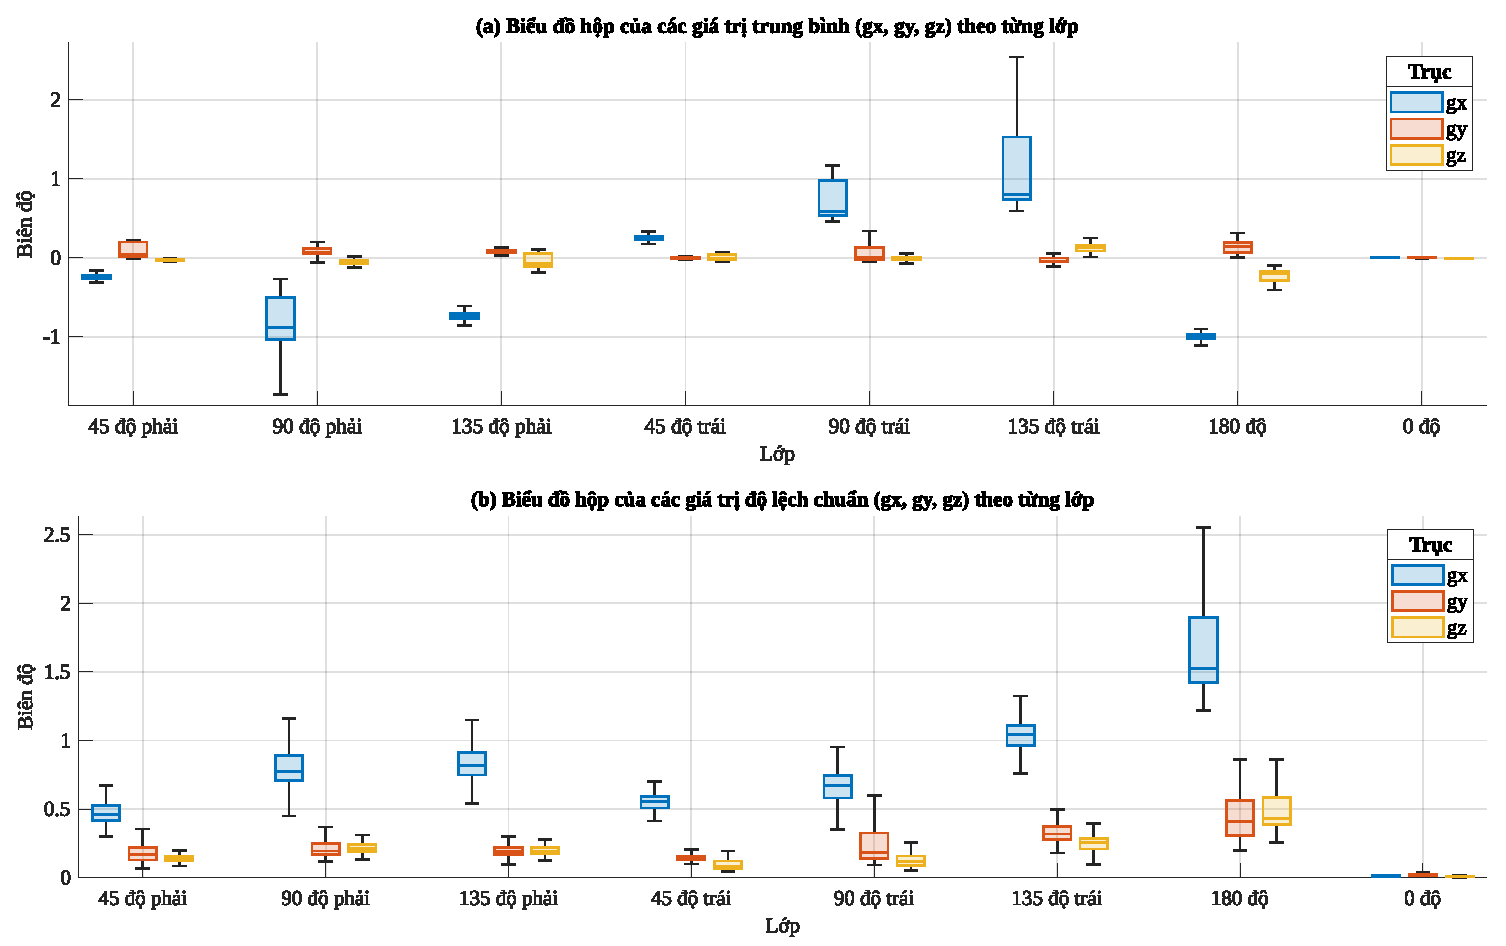
\includegraphics[width=1\linewidth]{Figure/gyro_boxplot_data.pdf}
    \caption{Phân bố giá trị trung bình và độ lệch chuẩn của dữ liệu con quay hồi chuyển ($\mathrm{g_x}$, $\mathrm{g_y}$, $\mathrm{g_z}$) theo từng hướng di chuyển}
    \label{gyro_boxplot_data}
\end{figure}

Tương tự như nhận dạng hành động, quy trình nhận dạng hướng di chuyển áp dụng cửa sổ trượt và các đặc trưng thống kê để phân đoạn dữ liệu con quay hồi chuyển thành các lớp chuyển động. Để trích xuất dữ liệu đầu vào cho mô hình phân loại, nhóm nghiên cứu sử dụng kỹ thuật cửa sổ động dựa trên phát hiện cực trị: tín hiệu rẽ trái được căn chỉnh theo đỉnh tín hiệu, còn tín hiệu rẽ phải được căn chỉnh theo đáy tín hiệu trên trục $\mathrm{g_x}$. Mỗi cửa sổ có độ dài cố định 150 mẫu và không có sự chồng lấp giữa các khung liên tiếp. Riêng với hướng đi thẳng 0$^\circ$, các cửa sổ được lấy liên tục với tỉ lệ chồng lấp 50~\% nhằm đảm bảo độ phủ đều trên chuỗi thời gian.

Nhằm đơn giản hóa mô hình và giảm tải tính toán, nghiên cứu lựa chọn hai đặc trưng thống kê cơ bản là trung bình và độ lệch chuẩn của tín hiệu con quay hồi chuyển trong từng cửa sổ thời gian. Hình~\ref{gyro_boxplot_data} cho thấy rõ sự phân tách giữa các lớp hướng di chuyển theo hai đặc trưng này—đặc biệt là trên trục $\mathrm{g_x}$—với xu hướng tăng/giảm có hệ thống tương ứng với từng mức độ quay. Cụ thể, giá trị trung bình phản ánh chiều và mức độ lệch tổng thể của chuyển động, trong khi độ lệch chuẩn thể hiện cường độ dao động trong quá trình xoay. Sự khác biệt nhất quán giữa các lớp cho thấy hai đặc trưng này đủ thông tin để mô hình học máy thực hiện phân loại hướng với độ chính xác cao mà không cần đến các đặc trưng phức tạp hơn.